\documentclass[11pt,a4paper]{report}

\usepackage{hyperref}
\usepackage{caption}
\usepackage{amsfonts}
\usepackage{cite}
\usepackage{graphicx}
\graphicspath{ {images/} }

\author{Catherine Vlasov}
\title{Optimizing Learning Parameters Used by Reinforcement Learning Algorithms}
\date{23 April 2018}


\begin{document}

\makeatletter
	\begin{titlepage}
		\vspace*{\fill}
		\begin{center}
			{\huge \bfseries \@title }
			\\[4ex]
			{\LARGE  \@author}
			\\[2ex]
			{\large \@date}
			\\[50ex]
			
\includegraphics[width=30mm]{oxlogo.png}
		\end{center}
		\vspace*{\fill}
	\end{titlepage}
\makeatother


%-----------------------
\begin{abstract}
This is my abstract
\end{abstract}


%-----------------------
\tableofcontents


%-----------------------
\chapter{Introduction}

Over the last few decades, reinforcement learning has seen a large increase in popularity. It amazes the world again and again, whether playing Go \cite{go}, Backgammon \cite{backgammon}, or Atari \cite{atari} games, and its potential continues to grow. These successes were not lucky, but rather they were a product of studying the nature, size, and complexity of each task, choosing the algorithm best suited to it, and then setting up the algorithm appropriately. The last of these steps is crucial to the success of reinforcement learning for a particular task and must be done carefully. Thus, this project aims to elucidate how to set up a reinforcement learning algorithm by tuning its parameters, specifically for a particular class of algorithms called Monte Carlo algorithms.


\section{Goals}

The specific Monte Carlo algorithm this project implements and investigates is called an ``on-policy $\varepsilon$-soft Monte Carlo control algorithm''. Section \ref{sec:Terminology} explains the basics of reinforcement learning as well as terminology used throughout this report, such as ``on-policy'' and ``$\varepsilon$-soft''. As the name suggests, the algorithm uses a parameter $\varepsilon$ to guide its learning. Effectively, it determines the balance between exploitation (choosing actions that are best, according to what it currently knows) and exploration (trying new actions). Thus, the chosen value of $\varepsilon$ can have a large effect on an agent's learning rate and therefore success at a particular task.

The on-policy $\varepsilon$-soft Monte Carlo control algorithm is not the primary subject of many research papers since it is simple, relative to other popular reinforcement learning techniques. Consequently, there is a lack of guidance on how to apply the algorithm to real tasks and achieve the greatest success given constraints such as computing power and time.

The simplicity of the algorithm, however, facilitates an interesting analysis of the effect of the value of $\varepsilon$ on the algorithm's success rate. The overarching goal of this project is to develop a general technique for tailoring the algorithm to a particular reinforcement learning task, which can then be extended to other reinforcement learning algorithms with parameters that need to configured.

This project tackles a number of questions:

\begin{itemize}
	\item Are there ``optimal'' values of $\varepsilon$ that maximise the algorithm's performance?
	\item How quickly does the algorithm's policy converge? Does it converge to the theoretical optimal policy?
	\item When playing games where states have axes of symmetry, how does the agent's 
performance and learning change when symmetry is eliminated?
	\item How does the performance of the algorithm differ for different games?
\end{itemize}

Three games were selected for this project: Tic-Tac-Toe, Chung Toi, and Nim. They are discussed in further detail in Section \ref{sec:DesignImpl}. They form an interesting mix since some have relatively long episodes, others can be used to investigate symmetry, and some with a similar state space can be compared against each other. Thus, it was possible to answer all of the above questions and derive some interesting results.



%-----------------------
\chapter{Background}

This section provides an overview of the theory behind reinforcement learning and the particular algorithm studied in this project.

\section{Reinforcement Learning}
\label{sec:RL}

Reinforcement learning (RL) is an area of machine learning in which an agent interacts with an environment by choosing actions, with the goal of maximizing the cumulative reward it receives for these actions.

The beauty of RL is that the agent is not given any information about \emph{how} to solve a problem, but rather it has to find out what works and what does not through trial-and-error. For this reason, RL is different from supervised learning because the agent is not provided with any input-output pairs to learn from. Instead, it learns and improves purely based on its own experiences.

RL is now described more formally. An \emph{agent} is a learner and the \emph{environment} is everything outside the agent, namely the thing that the agent interacts with. These interactions occur at discrete time steps $t = 0, 1, 2, 3, ...$. An \emph{episode} is a natural subsequence of interactions, such as a one game of Tic-Tac-Toe. There is a set of states $\mathcal{S}$ and a function $\mathcal{A}$ such that for any state $s \in \mathcal{S}$, $\mathcal{A}(s)$ is the set of actions that are available from state $s$. There is a function $\mathcal{R}$ that specifies the \emph{reward} (or \emph{return}) $r$ that an agent receives for choosing an action $a$ at a state $s$. The ultimate goal of an agent is to maximize the total sum of all the rewards it receives. Based on its experience, an agent builds a \emph{policy} $\pi$, which maps each state $s$ to the probabilities of selecting each of the actions available from $s$.

It is worth making a quick digression to explain what a Markov Decision Process (MDP) is. First, we define the \emph{Markov property}.

\begin{equation}
	\mathbb{P}(s_{t+1} = s', r_{t+1} = r \mid s_t, a_t, r_t, s_{t-1}, a_{t-1}, ... , r_1, s_0, a_0)
 \label{complete-prob-distr}
\end{equation}

\begin{equation}
	\mathbb{P}(s_{t+1} = s', r_{t+1} = r \mid s_t, a_t) \label{partial-prob-distr}
\end{equation}

A RL task has the Markov propety if and only if \ref{complete-prob-distr} and \ref{partial-prob-distr} are equal for all states $s'$, returns $r$, and all possible previous states, actions, and returns $s_t$, $a_t$, $r_t$, ... , $r_1$, $s_0$, $a_0$ \cite{rl-book}.

More intuitively, having the Markov property means that the environment's response (i.e. state it transitions to and return it gives to the agent) at a particular time step should only depend on what happened during the previous time step. Thus, this response should be independent of what happened before the previous time step.

A task that satisfies the Markov property is called a MDP and furthermore, if it has finitely many states and actions (i.e. $\mathcal{S}$ and $\mathcal{A}$ are both finite), then it is called a \emph{finite} MDP. 

The reason finite MDP's are important is that it has been shown that they all have an optimal policy $\pi^{\ast}$ \cite{rl-book}. Since the games used in this project all have finite state spaces and action spaces, this result is very useful since it facilitates the study of the convergence of an agent's policy as it gains experience playing the games.


\section{Learning Algorithms}

One of the goals of RL algorithms is to estimate a \emph{state-value function} that indicates the ``strength'' of being in a particular state. This ``strength'' refers to the expected return that the agent will receive from the environment if it follows a certain policy. Formally the state-value function for a policy $\pi$ is $V^{\pi} : \mathcal{S} \rightarrow \mathbb{R}$.

Similarly, RL algorithms also estimate an \emph{action-value function} that indicates the ``strength'' of choosing a particular action from a particular state. The action-value function for a policy $\pi$ is $Q^{\pi} : \mathcal{S} \times \mathcal{A} \rightarrow \mathbb{R}$.

RL algorithms estimate $V^{\pi}$ and $Q^{\pi}$ from experience and their goal is to build estimates as close to $V^{\ast}$ and $Q^{\ast}$ -- the optimal state-value and action-value functions -- as possible. We know that such optimal functions exist because, as explained in Section \ref{sec:RL}, all finite MDP's have an optimal policy.

A final distinction to make between RL algorithms is between \emph{on-policy} and \emph{off-policy} algorithms. On-policy algorithms update their estimates of the value functions solely using the experience they gain from choosing actions and interacting with the environment. On the other hand, off-policy algorithms update their estimates based on actions they might not even take.

There are a number of well-known RL techniques that estimate $V^{\pi}$ and improve policies in different ways. One of the most popular and well-understood \cite{challenges-of-rl} algorithms is Q-learning \cite{q-learning}, an off-policy algorithm. Most notably, a variant of Q-learning was used to train a convolutional neural network to play Atari 2600 games, outperforming human experts \cite{atari}. Q-learning is based in part on a category of RL algorithms called Temporal Difference, which are on-policy algorithms. One called TD($\lambda$) gained notoriety when it was successfully used to train a neural network to play Backgammon at a level that surpassed other similar networks as well as human experts \cite{backgammon}. Temporal Difference, in turn, combines techniques from dynamic programming approaches to RL as well another category of algorithms called Monte Carlo, which are mostly on-policy algorithms. The latter category is the focus of this project since such algorithms are simple and intuitive, but still reveal a lot about how policies converge and how performance varies from game to game.


\subsection{Monte Carlo Algorithms}
\label{sec:MonteCarloAlgorithms}

Monte Carlo (MC) algorithms are online algorithms that try to solve RL problems by computing the averages of returns. The term \emph{online} means that as the agent gains new information by interacting with the environment, this new information is immediately put to use. In particular, MC algorithms update their value function estimates and policies at the end of each episode. For this reason, MC algorithms are only used for tasks that can be divided into discrete episodes that are guaranteed to terminate eventually.

MC learning works by saving the average of all returns received for choosing action $a$ from $s$, for each state $s$ and action $a$ available from $s$, over the course of all episodes. This is stored in the action-value function $Q^{\pi}$.

There are two variations of MC with respect to averaging returns: \emph{every-visit} MC and \emph{first-visit} MC. Every-visit MC computes its estimate of each expected return $Q(s,a)$ using the average of the returns after \emph{all} the times $a$ was chosen from $s$. In contrast, first-visit MC does so using only the returns received the \emph{first} time $a$ was chosen from $s$ in each episode. Both versions converge to the true expected values in the limit of infinitely many encounters with each state-action pair, so the first-visit version was arbitrarily chosen for this project.

A problem arises when a policy is completely deterministic because many state-actions pairs will never be encountered, regardless of how many episodes take place. More specifically, only one action from each state will be chosen whenever the state is encountered, so the algorithm will never improve. Thus, a concept called \emph{exploring starts} is assumed. This means that the each episode begins with a random state-action pair, where all pairs have a non-zero probability of being selected. In this way, all states and actions are guaranteed to be encountered infinitely many times over the course of infinitely many episodes.

However, exploring starts cannot be assumed to hold for all RL tasks and one solution to this problem is an on-policy control method. Policies resulting from these methods are called \emph{$\varepsilon$-soft} if $\pi(s,a) > 0$ for all $s \in \mathcal{S}$ and all $a \in \mathcal{A}(s)$. A specific type of $\varepsilon$-soft policy is an $\varepsilon$-greedy policy and this is the type used in this project. The way they work is that the majority of the time, the agent chooses the best action, but with probability $\varepsilon$ it chooses an action randomly. Specifically, the best action is assigned a probability of $1 - \varepsilon + \frac{\varepsilon}{|\mathcal{A}(s)|}$ and all other actions are assigned a probability of $\frac{\varepsilon}{|\mathcal{A}(s)|}$ in the policy.

With all of this in mind, we can now understand the on-policy $\varepsilon$-soft MC control algorithm used in this project:

\label{sec:monteCarloPseudocode}
\begin{center}
	\emph{[will figure out how to use the algorithm package to write pseudocode here]}
\end{center}


\section{Terminology}
\label{sec:Terminology}

In addition to the terms described in Section \ref{sec:RL}, the following terms are used throughout this project:

\begin{itemize}

	\item \textbf{Random agent}: Agent that randomly chooses an action from the list of available actions at any given state
		\begin{itemize}
			\item In particular, an instance of the \emph{RandomAgent} class described in Section \ref{sec:Agents})
		\end{itemize}

	\item \textbf{MC agent}: Agent that uses the on-policy $\varepsilon$-soft Monte Carlo control algorithm for learning
		\begin{itemize}
			\item In particular, it refers to an instance of the \emph{MonteCarloAgent} class described in Section \ref{sec:Agents}
		\end{itemize}

	\item \textbf{Game}: Examples are Tic-Tac-Toe, Connect Four, and Chess

	\item \textbf{Training episode}: Making a MC agent play one iteration of a game for the purposes of learning/training

	\item \textbf{Training session}: Running some number of training episodes consecutively (e.g. ten thousand, one million)

\end{itemize}


%-----------------------------------------
\chapter{Design \& Implementation}
\label{sec:DesignImpl}

This section describes the implementations of Tic-Tac-Toe, Chung Toi, and Nim, as well as the game-playing agents used in this project's experiments.


\section{Structure}

The project is written entirely in Java and is built in a modular way, using an object-oriented style. All actions, agents, games, and states implement general interfaces, called \emph{Action}, \emph{Agent}, \emph{Game}, and \emph{State} respectively, that serve as Facades for the complex implementations. Figure \ref{code-structure} shows this structure.

\begin{figure}[htbp]
	\begin{center}
		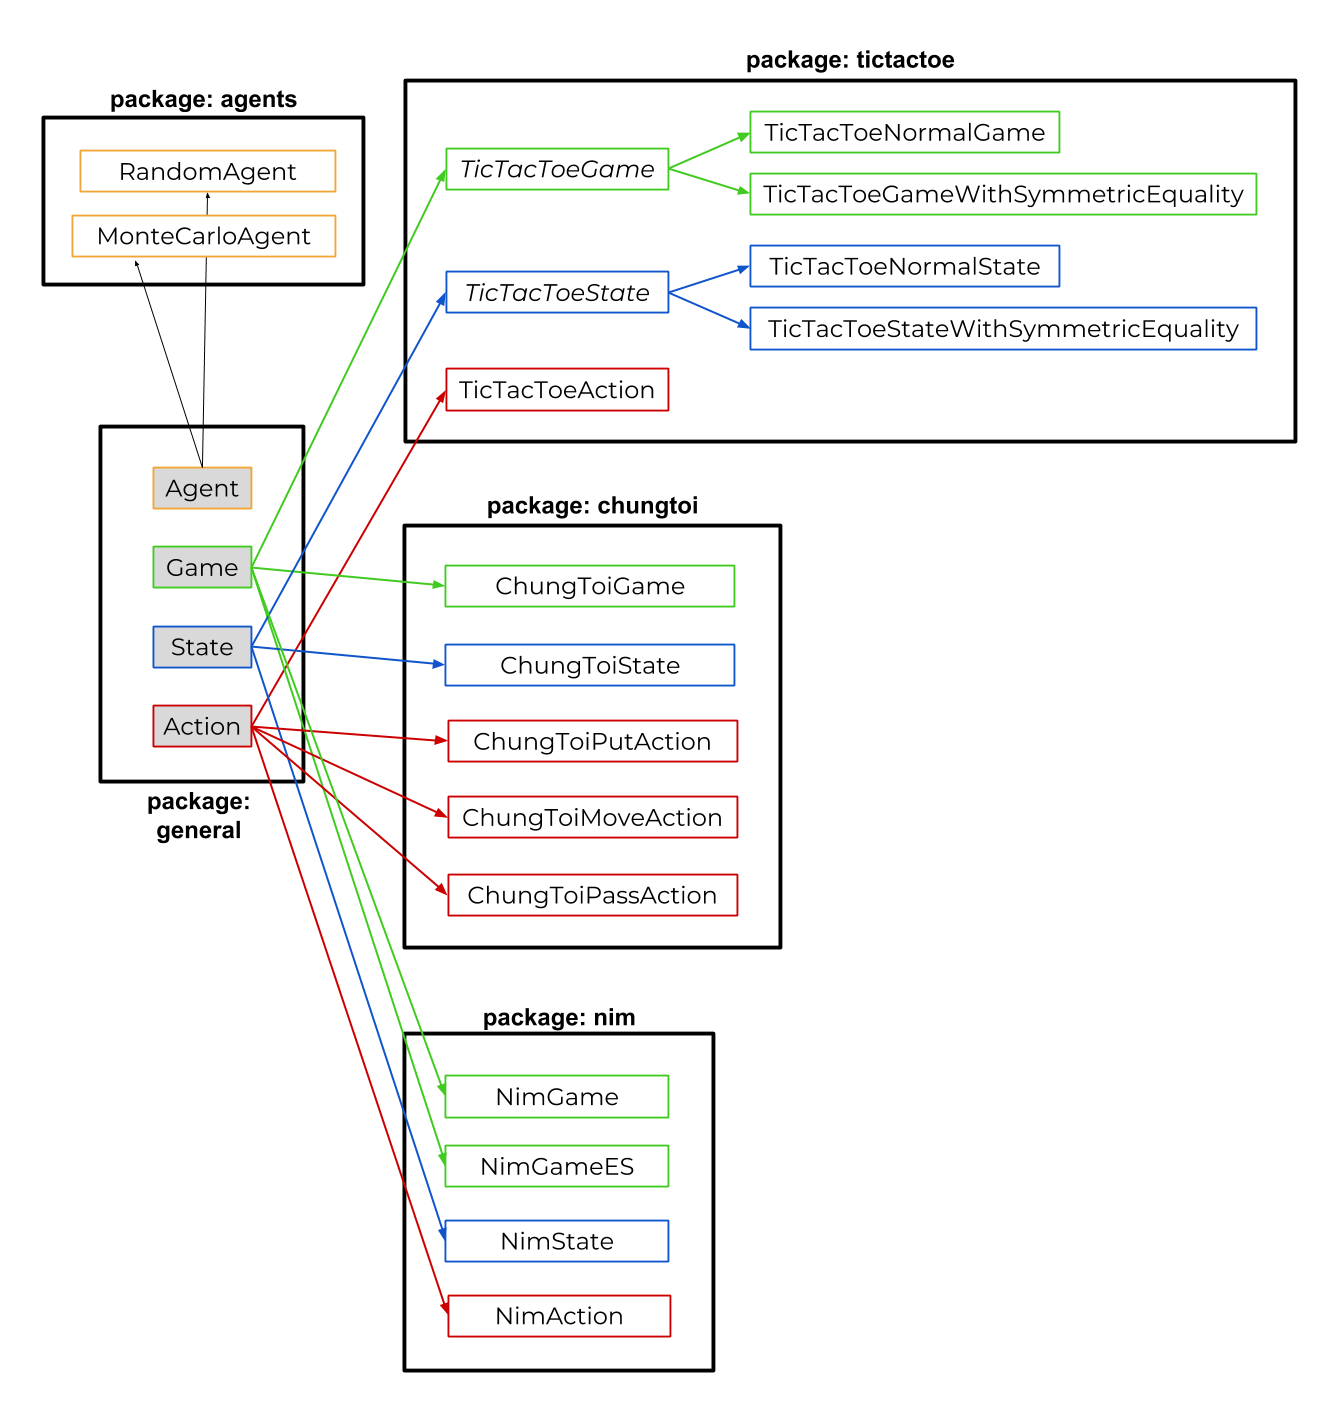
\includegraphics[width=125mm]{code_structure.png}
		\caption{Structure of classes in project.}
		\label{code-structure}
	\end{center}
\end{figure}

The \emph{Game} interface has a method \emph{play()} that simulates a single game. This is where the agents are asked to choose actions, receive returns, and complete other tasks, depending on the specific game. Agents do not distinguish between different games and only use methods defined in the general interfaces, which means that the \emph{MonteCarloAgent} class, for example, can be used to play all three games. This modularity provides a nice separation of concerns that enables simpler testing and debugging.


\section{Agents}
\label{sec:Agents}

Two agents were implemented: \emph{RandomAgent} and \emph{MonteCarloAgent}.

\emph{MonteCarloAgent} implements the $\epsilon$-soft on-policy MC control algorithm, as discussed in Section \ref{sec:MonteCarloAlgorithms}. In its \emph{chooseAction(State s)} method, it chooses an action according to its policy for states it has encountered in previous games, and randomly otherwise. In its \emph{gameOver()} method it calls two private helper methods \emph{policyEvaluation()} and \emph{policyImprovement()} that update $Q^{\pi}$ and $\pi$, respectively, as described in Section \ref{sec:monteCarloPseudocode}. Hash maps are used to store $Q^{\pi}$ and $\pi$ for constant time access and insertion.

As its name suggests, \emph{RandomAgent} randomly selects an action from the list of available actions at any given state. In total, the logic for this agent is equivalent to one line of code and this agent is only used to play against the MC agent during training.


\section{Tic-Tac-Toe}
\label{sec:TicTacToe}

The first game used in this project is Tic-Tac-Toe. It was chosen as a first experiment because it has a small state space and it is a conceptually simple game that most people are familiar with.


\subsection{Rules}

Although this is a widely-known game, the rules \cite{tic-tac-toe-rules} are still included here for reference and clarity.

First, one of the two players is randomly selected to use X tokens (the other player uses O tokens). These players are referred to as the ``X-player'' and ``O-player'', respectively, and they both have an unlimited number of tokens at their disposal. The game then consists of the two players alternately placing their tokens in empty spaces on a 3x3 grid, starting with the X-player. Figure \ref{tic-tac-toe-grid-example} is an example of a possible state of the grid.

\begin{figure}[htbp]
	\begin{center}
		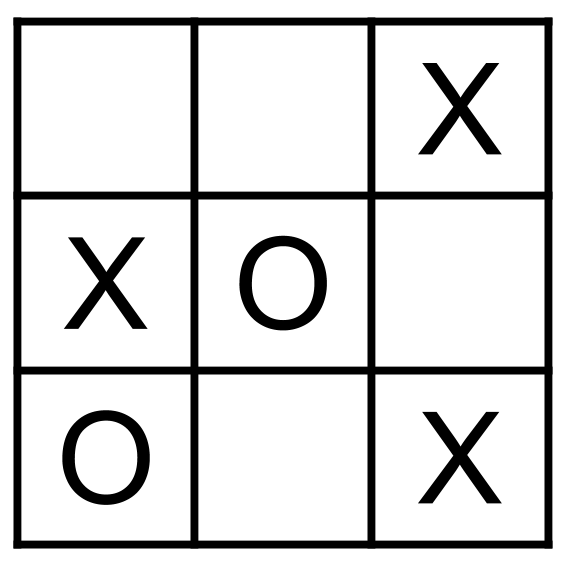
\includegraphics[width=50mm]{tictactoe_grid_example.png}
		\caption{Example of a Tic-Tac-Toe grid. Each of the nine cells can be in one of three states: empty, X, or O.}
		\label{tic-tac-toe-grid-example}
	\end{center}
\end{figure}

The game has three possible endings:

\begin{itemize}
	\item \textbf{X-player wins}: three X tokens form a horizontal, vertical, or diagonal row
	\item \textbf{O-player wins}: three O tokens form a horizontal, vertical, or diagonal row
	\item \textbf{Draw}: the grid is filled and neither player has won
\end{itemize}


\subsection{State Space}
\label{sec:TicTacToeStateSpace}

Since each cell has three possible states, there are at most $3^9 = 19683$ states. In practice, strictly fewer than 19,683 possible states can be reached because technically the grid can be filled only with X tokens, with more O tokens than X tokens, or even with a row of three X tokens \emph{and} a row of three O tokens. None of these examples are valid game states so none of them will ever be encountered in a real game.

Preliminary experiments reveal that, in fact, only 4520 states are reachable, without taking into account the four axes of symmetry of a Tic-Tac-Toe grid. If these are taken into account, we find that there are only 640 unique (quotiented by equality by symmetry) reachable states.


\subsection{Implementation}
\label{sec:TicTacToeImplementation}

One of the aims of this project is to investigate the effect of eliminating a game's state symmetries on the Monte Carlo algorithm's learning rate and optimal learning parameters. In the game of Tic-Tac-Toe, a state can be symmetrical with up to seven other states as result of flipping it in the following ways:

\begin{itemize}
	\item horizontal axis
	\item vertical axis
	\item horizontal axis then vertical axis
	\item major diagonal (i.e. top left to bottom right)
	\item major diagonal then horizontal axis
	\item minor diagonal (i.e. top right to bottom left)
	\item minor diagonal then horizontal axis
\end{itemize}

Of course, for some states, the result of some of these flips are the same, which is why a state might have strictly less than seven other symmetrical states.

With this goal in mind, Tic-Tac-Toe was implemented in two ways:

\begin{itemize}

	\item \textbf{``Normal''}:
This version does not break any symmetry and was used as a baseline.

	\item \textbf{``Symmetric Equality''}: 
This version breaks the symmetry between states by considering two objects representing states to be ``equal'' if they are symmetrical.

\end{itemize}

Implementing the desired behaviour for the Symmetric Equality version was not as simple as initially expected. Overriding the \emph{equals()} method inherited from Java's \emph{Object} class was straightforward. However, overriding the inherited \emph{hashCode()} method was tricky.

A Java \emph{HashMap} places key-value pairs in buckets depending on the value returned by calling \emph{hashCode()} on the keys. Thus, if two keys have different hash codes, then they are placed in two different buckets, even if they are ``equal'' according to both of their \emph{equals()} methods. So, two key-value pairs with ``equal'' keys can both end up being stored in a hash map at the same time if they have different hash codes. This is why it was crucial for the \emph{hashCode()} method in \emph{TicTacToeStateWithSymmetricEquality} to produce exactly the same result for symmetrical states. After considering a few solutions, this behaviour was ultimately implemented by silently converting each state to a canonical form in such a way that symmetrical states have the same canonical form. Each state's canonical form is used to compute the state's hash code, which results in all symmetrical states having the same hash code, as required.

In both Tic-Tac-Toe implementations, agents receive a return of 1 for an action resulting a win, -1 for an action resulting in a loss, and 0 for an action resulting in a draw or a non-terminal state.


\section{Chung Toi}
\label{sec:ChungToi}

The second game used in the project is Chung Toi, a more complex version of Tic-Tac-Toe that has been studied in the context of reinforcement learning \cite{chung-toi-rl}. Its state space is larger than that of Tic-Tac-Toe which leads to interesting results.


\subsection{Rules}

The main idea behind Chung Toi \cite{chung-toi-rules} is the same as that behind Tic-Tac-Toe in the sense that the game is played on a 3x3 grid and each player's goal is to get three of their pieces in a row. However, that is the entire extent of their overlap. Although the two games may seem similar, finding a good strategy for Chung Toi is not at all intuitive, unlike in Tic-Tac-Toe.

Before the game begins, one of the two players is randomly selected to use red tokens (the other player uses white tokens). These players are referred to as the ``red player'' and ``white player'', respectively. Each player has three tokens at their disposal and each token can be used in two possible orientations, as shown in Figure \ref{chung-toi-tokens}.

\begin{figure}[htbp]
	\begin{center}
		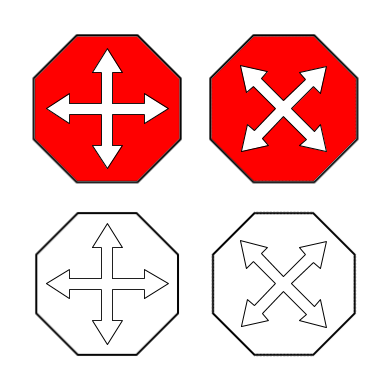
\includegraphics[width=40mm]{chung_toi_tokens.png}
		\caption[Chung Toi tokens]{Red and white Chung Toi tokens in both possible orientations. The tokens in these orientations are referred to as: red-straight (top-left), red-diagonal (top-right), white-straight (bottom-left), and white-diagonal (bottom-right).}
		\label{chung-toi-tokens}
	\end{center}
\end{figure}

The game consists of the players alternately making a move, starting with the red player. Throughout the game, the red player can only move red tokens and the white player can only move white tokens. The game has two phases and both players start in Phase 1. Once a player places all three of their tokens, that player proceeds to Phase 2. The following actions are available in each phase:

\begin{itemize}

	\item \textbf{Phase 1}
		\begin{itemize}
			\item Place a token (in either orientation) in an empty grid cell
			\item Pass
		\end{itemize}

	\item \textbf{Phase 2}
		\begin{itemize}
			\item Slide a token on the grid in the direction of any of the arrows on that token. When the token reaches the final cell, it can be rotated to switch its orientation if the player chooses to do so. \emph{(Note: all grid cells in the path from the original cell to the final cell must be empty, meaning that the token cannot ``jump'' over other tokens)}
			\item Rotate one token to switch its orientation
			\item Pass
		\end{itemize}

\end{itemize}

If both players pass on consecutive turns at any point, the game ends and is declared a draw. Otherwise, the game continues until one of the players makes their tokens form a horizontal, vertical, or diagonal row and that player is declared the winner. The orientation of the three tokens in the row does not matter.

Figure \ref{chung-toi-grid-example} is an example of a possible state of the grid.

\begin{figure}[htbp]
	\begin{center}
		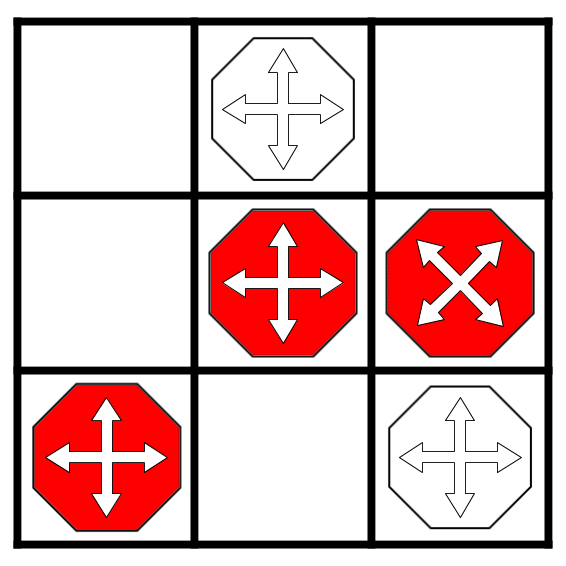
\includegraphics[width=50mm]{chung_toi_grid_example.png}
		\caption{Example of a Chung Toi grid. Each of the nine cells can be in one of five states: empty, red-straight, red-diagonal, white-straight, or white-diagonal.}
		\label{chung-toi-grid-example}
	\end{center}
\end{figure}


\subsection{State Space}

Since each cell has five possible states, there are at most $5^9 = 1,953,125$ states. For the same reasons outlined in Section \ref{sec:TicTacToeStateSpace}, strictly fewer than this many states are reachable in practice and even fewer are unique with respect to the four axes of symmetry.


\subsection{Implementation}

A standard implementation of Chung Toi was developed for this project. It enables two agents to play the game, exactly as described above.

The role of Chung Toi in this project was to learn more about the effect of the MC learning parameter $\varepsilon$ on an agent's learning rate and winning rate. Chung Toi has roughly 100 times more states than Tic-Tac-Toe, which is expected to have an effect on the optimal value of $\varepsilon$ and therefore the MC agent's learning rate. It has the same axes of symmetry as Tic-Tac-Toe, so similar results would be expected from a Chung Toi implementation that breaks symmetries. For this reason, such an implementation was not developed to reduce redundancy and instead only a normal implementation with all symmetrical states present was developed.

Just like in Tic-Tac-Toe, agents receive a return of 1 when they win, -1 when they lose, and 0 when the game ends in a draw or the game has not yet ended.


\section{Nim}
\label{sec:Nim}

The third game used in the project is Nim, a simple game with an interesting mathematical theory behind it \cite{nim-rules}. It has a large number of variations and can be configured in many ways, so its state space can vary widely. For the purposes of this project, a ``small'' version of the game is used in order to reduce the running time of the experiments.


\subsection{Rules}

The general idea of Nim \cite{nim-rules} is that two players alternately remove objects from several piles. The first player is chosen randomly and then on each turn, a player can remove any number of objects from any one of the piles. Each player must remove at least one object on each turn. The game ends when all the piles are empty.

Which player wins depends on which version of the game is being played. In the ``normal play'' version the last move is the winning move, whereas in the ``mis\`ere'' version the player who moves last loses \cite{winning-ways-math-plays}. The mis\`ere version is implemented in this project.


\subsection{State Space}

As explained in Section \ref{sec:NimImplementation}, the ``small'' version of Nim used in this project  consists of three piles, initially with seven objects each. Since each pile can have between zero and seven objects, inclusive, there are $8^3 = 512$ possible states.


\subsection{Implementation}
\label{sec:NimImplementation}

Nim is traditionally played with three piles of objects. The first of two versions of Nim implemented in this project is standard and initialises all piles with a fixed number of objects. In particular, in order to keep the state space relatively small, all three piles start off with seven objects.

A second version of Nim was implemented since the game is well-suited to investigating the performance of Monte Carlo ES. This is because instead of initialising all piles with a fixed number of objects, all piles can be initialised with random numbers of objects.

In this second implementation, piles are initialised with a random number of objects between zero and seven, in such a way that at least two piles are non-empty. This last condition was necessary because if all piles are empty or if there is only one non-empty pile and the other agent goes first and removes all the objects, then the game ends and the MC agent must receive a return without having chosen any action. This creates problems in the policy improvement phase of the algorithm since there is an outstanding return relative to the number of actions taken (i.e. zero).

Since the concept of exploring starts relies on games starting with random state-action pairs, the implementation of the MC agent (as well as the \emph{Agent} interface and random agent) had to be modified and a slightly modified version of Nim was created. This is because in addition to randomly initialising the piles, an action has to be randomly selected. Then, the agent that is randomly selected to go first has to be forced to choose that random action. In this way, in the limit of infinitely many games, all actions from all states are explored and the agent is able to determine the overall best return it can receive from each state.

At the end of the game, the winner receives a return of 1 and the loser receives a return of -1. Throughout the rest of the game, both players receive returns of 0 for all their actions.


%------------------
\chapter{Results \& Analysis}

This section describes the outcomes of a variety of experiments and discusses why these outcomes were expected, or unexpected, and what can be learned from them.


\section{Types of Experiments}

Two types of experiments were used to investigate the behaviour of the MC agent when playing games:

\begin{itemize}

	\item \textbf{``Epsilon'' Experiment}: This type of experiment iterates through all values of epsilon in a particular range and makes a MC agent (initialised with each value of epsilon) play a specific game against itself or another agent a fixed number of times. Then it records the results (i.e. wins, losses, draws) for each value of epsilon in a CSV file. Thus, it is possible to produce graphs with the tested values of epsilon on the x-axis and the number of episodes resulting in a win, loss, and draw on the y-axis. These graphs are used to determine the optimal value of epsilon for a particular game.

	\item \textbf{``Convergence'' Experiment}: This type of experiment makes a MC agent (initialised with a particular value of epsilon) play a specific game against itself or another agent a fixed number of times. In the process, it records the cumulative results (i.e. wins, losses, draws) at regular intervals, as more and more games are played, in a CSV file. Thus, it is possible to produce area charts with the cumulative number of games on the x-axis and percentages on the y-axis to show the proportions of wins, losses, and draws. These graphs are used to visualise the convergence rate of a MC agent's policy when using a specific value of epsilon.

\end{itemize}

The data from running these experiments on different games and with agents playing against each other different numbers of times was combined to produce a number of interesting graphs that reveal interesting properties of the Monte Carlo control algorithm used.


\section{Number of Training Episodes}

One decision that was made in the design and execution of these experiments was the number of training episodes to make a MC agent play for each experiment type and each game. Through a process of trial-and-error, it was determined that for Tic-Tac-Toe and Chung Toi, the agent needed at least 10,000 training episodes before having it would be able to reach a reasonable portion of the states. For Nim, 1,000 training episodes was determined to be a good starting point.


\section{Optimal Value of $\varepsilon$}

It is not unreasonable to expect each game to have a specific value of epsilon that results in the fastest convergence of the learning agent's policy. If this was the case, then one would expect the graph of the winning rate produced by an epsilon experiment with $\varepsilon$ ranging from 0.0 to 1.0 (inclusive) to be convex with a global maximum. This belief is vaildated by running an epsilon experiment on any game for some number of training games. For example, Figure \ref{chung-toi-epsilon-1M-graph} displays the results of training a MC agent on one million episodes of Chung Toi.

\begin{figure}[htbp]
	\begin{center}
		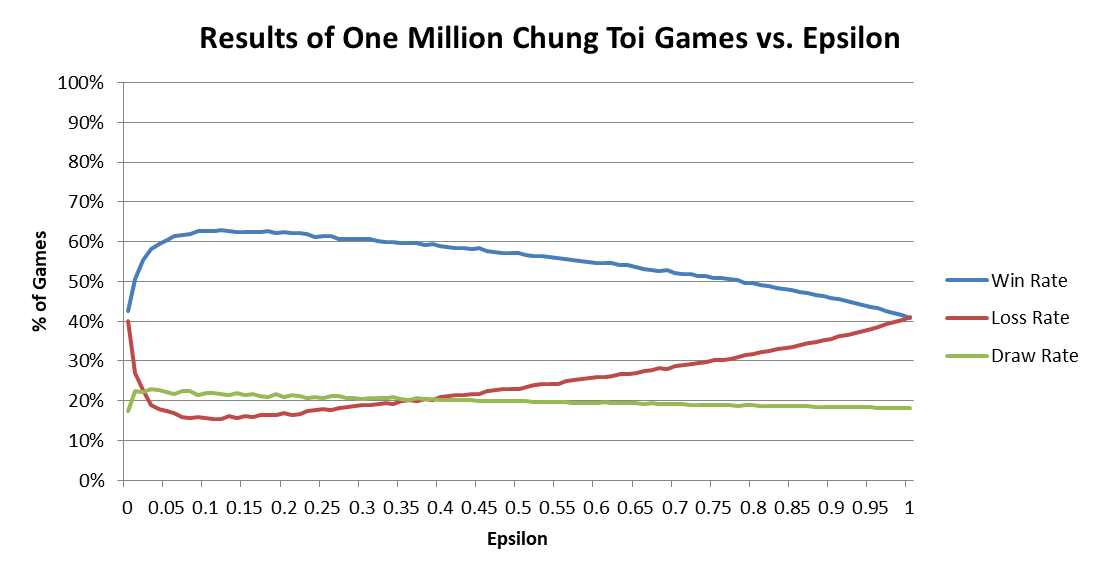
\includegraphics[width=125mm]{ChungToi_EpsilonResults_1MGames.png}
		\caption{Results of training learning agent with one million episodes of Chung Toi}
		\label{chung-toi-epsilon-1M-graph}
	\end{center}
\end{figure}

However, with some experimentation it becomes clear that there is another key factor in the equation: the number of training episodes. If a game is judged based on the results of a single epsilon experiment (which runs some number of training episodes), the belief that each game has an optimal epsilon value seems to be true. However, when many epsilon experiments that run different numbers of training episodes are considered, an interesting relationship between the number of training episodes and the optimal value of epsilon is uncovered. Figure \ref{nim-epsilon-win-comparison} demonstrates this relationship for Nim. The same relationship is also visible in the graphs for Tic-Tac-Toe and Chung Toi.

\begin{figure}[htbp]
	\begin{center}
		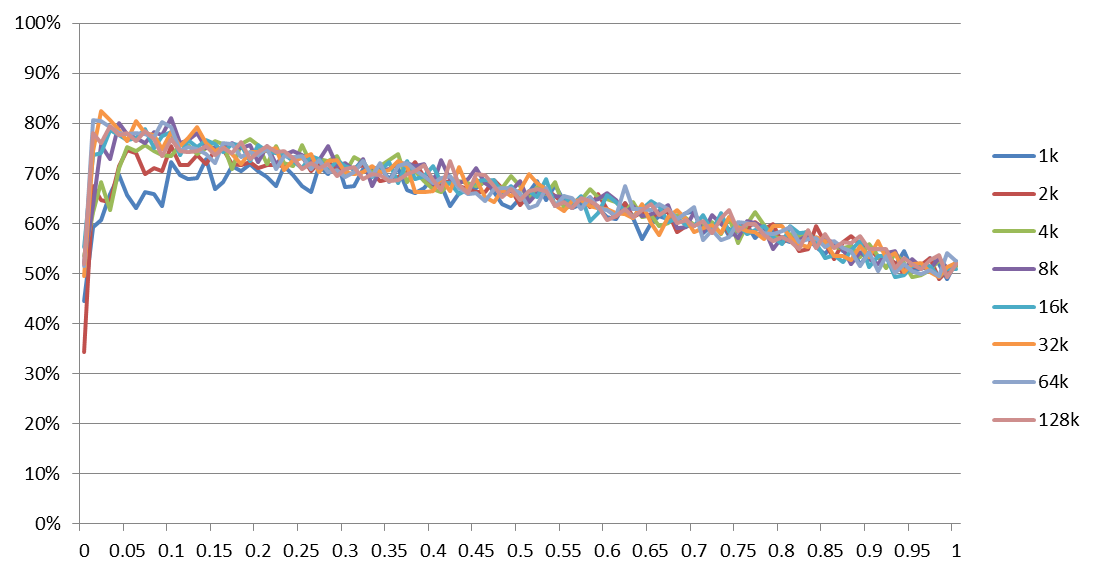
\includegraphics[width=125mm]{Nim_EpsilonResults_Wins_Comparison.png}
		\caption{Comparison between results from different numbers of training episodes for Nim}
		\label{nim-epsilon-win-comparison}
	\end{center}
\end{figure}

Thus, as the number of training episodes increases, the optimal value of epsilon decreases and approaches zero. In particular, if we plot the optimal value of epsilon against the number of training episodes, for any game, we get a graph that looks like Figure \ref{nim-training-vs-opt-epsilon}, which exhibits an inverse relationship \textbf{(??)} between the two. In order to obtain more accurate optimal epsilon values for Figure \ref{nim-training-vs-opt-epsilon}, each epsilon experiment was run three times and the results were averaged. \textbf{[\emph{In this particular version, the experiment was only run once -- I will run it twice more to make a smoother graph}]} % NEED TO DO THIS

\begin{figure}[htbp]
	\begin{center}
		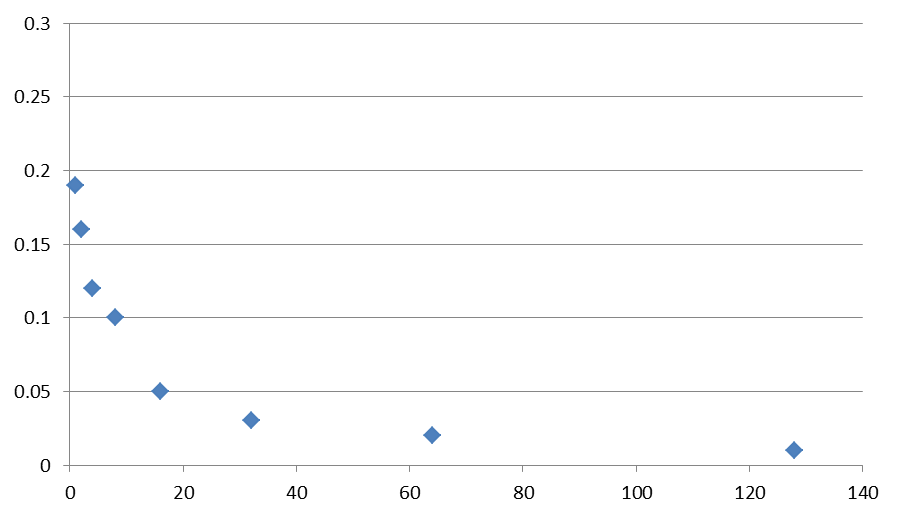
\includegraphics[width=125mm]{Nim_OptimalEpsilon_vs_Training.png}
		\caption{Relationship between optimal epsilon value and number of training episodes for Nim}
		\label{nim-training-vs-opt-epsilon}
	\end{center}
\end{figure}

This behaviour actually makes sense and should, in fact, be expected because of the role of $\varepsilon$ in the Monte Carlo control algorithm. As discussed in Section \ref{sec:MonteCarloAlgorithms}, $\varepsilon$ is used during policy improvement. In particular, the probability of choosing an action (other than the best action encountered so far) is $\frac{\varepsilon}{N}$ where $N$ is the number of available actions. On the other hand, the probability of choosing the best action encountered so far is  $1 - \epsilon + \frac{\varepsilon}{N}$. Thus, as $\varepsilon$ approaches zero, the probability of choosing the best action encountered so far approaches one.

As the number of training episodes approaches infinity, the probability that the agent has encountered the best actions for all states approaches 1. Once the best action from a state has been encountered, the agent no longer benefits from randomly trying other actions since doing so can only lead to smaller (or equal) returns. Therefore, from then on, the agent will earn the largest overall return by choosing the best action from that state with a very large probability whenever that state is encountered.

A larger value of $\varepsilon$ benefits an agent in the short-term because it speeds up learning. This is because a larger $\varepsilon$ value corresponds to more exploration, relative to exploitation, which means the best actions will be found faster. However, it is disadvantageous in the long-term because even though the agent knows which actions produce the largest returns, the agent will still be forced to choose other actions relatively often.

Overall, there is no single value of $\varepsilon$ that maximises an agent's performance in a particular game. However, for any \emph{specific} number of training episodes, there \emph{is} a value that results in the best winning rate by striking the right balance between exploration and exploitation for \emph{that} amount of training.

[\emph{Maybe mention that optimal values vary from game to game due to varying state spaces. Also I could briefly mention why the behaviour at 0.0 and 1.0 is the same in all experiments.}]


\section{Convergence to the Optimal Policy}

In the context of training a MC agent to play a game, the ``speed'' at which the agent's policy converges is the number of training episodes the agent needs until its policy $\pi$ converges. Naturally, this varies depending on the value of $\varepsilon$ used by the agent.

The policy of the MC agent only converges to the theoretically optimal policy in the limit of infinitely many training episodes \cite{rl-book}. Since running infinitely many episodes is naturally infeasibly, in this project we consider the policy to have converged after $x$ training games if the agent's winning rate changes by less than 0.1\% after $x$ training episodes compared to after $x+1000$ training episodes.

In the experiment framework developed for this project, convergence experiments provide the data needed to compare different values of $\varepsilon$ and to analyse the speed of convergence. Convergence experiments produce the proportions of wins and losses (and draws, if applicable) at regular intervals as an agent participates in more and more training episodes, using a specific value of epsilon. Thus, by plotting these ratios as an area chart and looking at the borders between the regions, we see how quickly the policy changes.

For instance, in Figure \ref{nim-epsilon-win-comparison}, we see that the agent's winning rate when playing Nim changes quite significantly as the number of training episodes increases. We can also see that using $\varepsilon = 0.1$ seems to make the agent perform relatively well. This suggests that running a convergence experiment for Nim with $\varepsilon = 0.1$ might provide insight into the policy's convergence rate. Figure \ref{nim-0-1-convergence} shows these results.

\begin{figure}[htbp]
	\begin{center}
		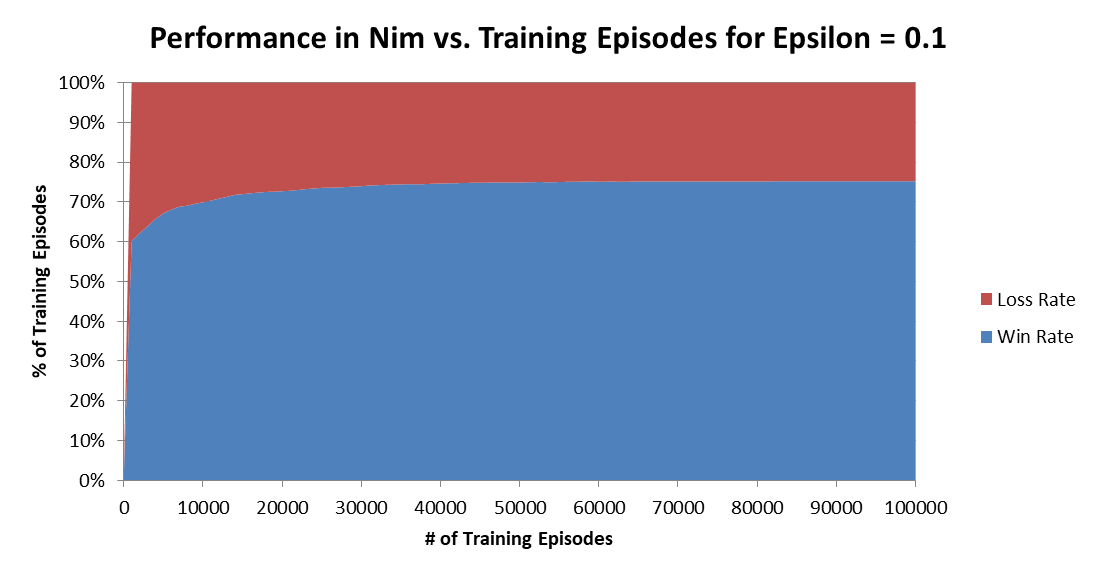
\includegraphics[width=125mm]{Nim_PerformanceResults_0_1.png}
		\caption{Changes in agent's performance in Nim with $\varepsilon = 0.1$}
		\label{nim-0-1-convergence}
	\end{center}
\end{figure}

As we can see, after aroud 20,000 training episodes, the agent's performance stabilises. In fact, the performance (and therefore policy) converges -- by this project's definition of convergence -- after $19,000$ training episodes.

On the other hand, Figure \ref{nim-epsilon-win-comparison} shows that the agent's winning rate in Nim for values of epsilon larger than 0.5 does not not change significantly as the number of training episodes increases. So, we expect the agent's policy to converge faster. This intuition is confirmed by Figure \ref{nim-0-5-convergence}, which shows the results of a convergence test for Nim with $\varepsilon = 0.5$. Specifically, the policy converges after only $7,000$ training epsidodes.

\begin{figure}[htbp]
	\begin{center}
		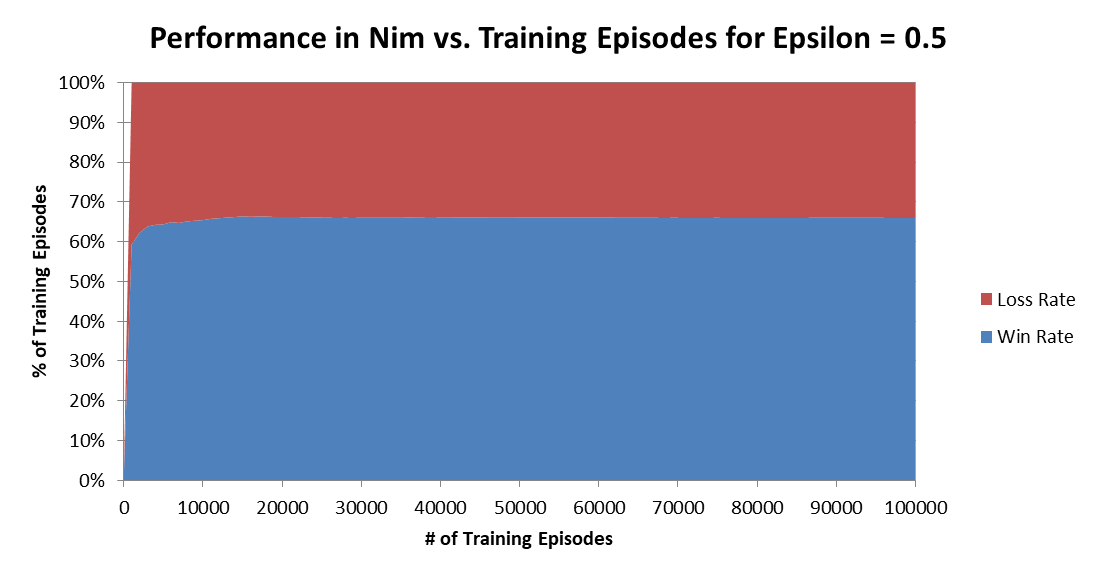
\includegraphics[width=125mm]{Nim_PerformanceResults_0_5.png}
		\caption{Changes in agent's performance in Nim with $\varepsilon = 0.5$}
		\label{nim-0-5-convergence}
	\end{center}
\end{figure}

Finally, the part of Figure \ref{nim-epsilon-win-comparison} that shows the most variation is where epsilon is very small. Figure \ref{nim-0-01-convergence} displays the results of a convergence experiment for Nim with $\varepsilon = 0.01$. This shows that the policy takes much longer to converge -- $42,000$ training episodes, to be precise.

\begin{figure}[htbp]
	\begin{center}
		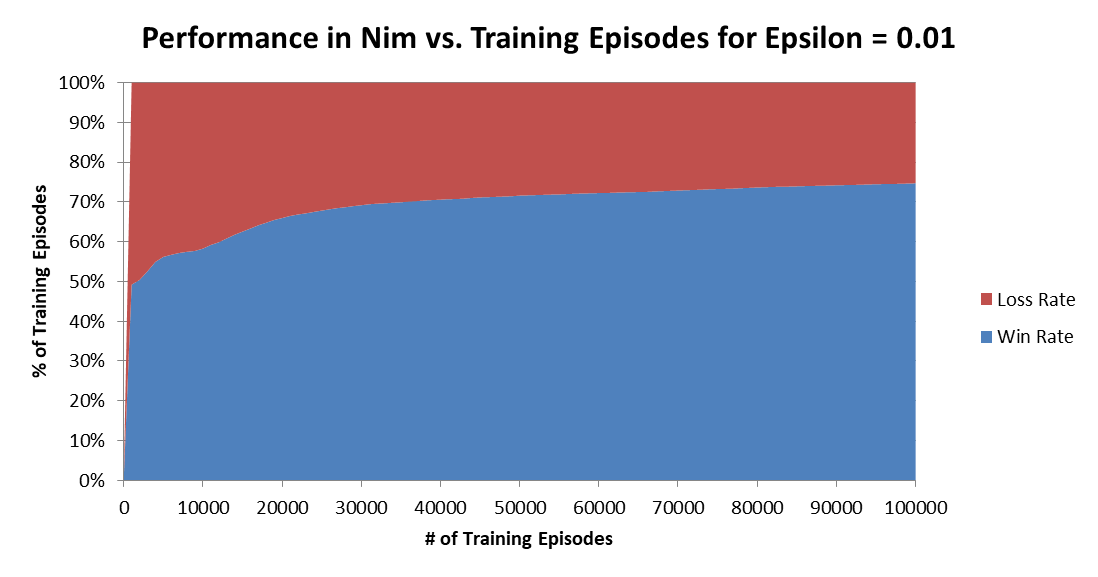
\includegraphics[width=125mm]{Nim_PerformanceResults_0_01.png}
		\caption{Changes in agent's performance in Nim with $\varepsilon = 0.01$}
		\label{nim-0-01-convergence}
	\end{center}
\end{figure}

Convergence experiments were run on several values of epsilon and the results are summarised in Table \ref{table:nim_convergence_table}. As we can see, the results empirically verify the following intuitions:

\begin{itemize}

	\item \textbf{$\varepsilon$ should not be too small (otherwise new actions will rarely be chosen) or too large (otherwise the best actions will rarely be chosen).} This is indeed the case since the best value of epsilon is not quite at either extreme of the range of values tried. For Nim, the value with the largest winning rate at convergence is $\varepsilon = 0.04$.

	\item \textbf{In general, as $\varepsilon$ gets larger, the number of training episodes until convergence decreases.}

	\item \textbf{As $\varepsilon$ gets larger, the agent is more likely to encounter all possible states (assuming a reasonably small state space).} This is clearer when looking at Table \ref{table:nim_convergence_table}, which shows the actual data produced by the convergence experiments since it shows how many states were encountered after every additional 1,000 training episodes. Looking at the detailed results in the CSV file produced by the experiment, we can see event more: in the case of $\varepsilon = 0.64$ all states were encountered after only 5,000 episodes whereas it took tens of thousands of episodes for the smaller values of $\varepsilon$ that were tested.

\end{itemize}

\begin{table}[ht]
	\centering
	\begin{tabular}{c c c c}
		Epsilon & Training Episodes & States Encountered & Winning Rate \\
		\hline
		0.01 & 42,000 & 494 & 70.7\% \\
		0.02  & 47,000 & 507 & 75.7\% \\
		0.04  & 38,000 & 511 & 76.5\% \\
		0.08  & 21,000 & 508 & 76.1\% \\
		0.16  & 19,000 & 507 & 72.7\% \\
		0.32  & 9,000 & 509 & 70.4\% \\
		0.64 & 8,000 & 511 & 61.5\% \\
	\end{tabular}
	\caption{Data About Nim Policy Convergence for Multiple Values of Epsilon}
	\label{table:nim_convergence_table}
\end{table}


\section{Monte Carlo with Exploring Starts}

The game that is most conducive to applying the Monte Carlo with exploring starts algorithm is Nim because it is easy to create a random starting state. Since Monte Carlo with exploring starts does not have any learning parameters like $\varepsilon$, the only relevant type of experiment is a convergence experiment. Normally, a convergence experiment takes a value of $\varepsilon$ as an argument, but since such a value is not used by an agent that implements the exploring starts algorithm, the argument is ignored. Thus, the only experiment parameter that can be modified is the total number of training episodes. For consistency with the other experiments on Nim, the convergence experiment for Nim with exploring starts was run 100,000 times and the results can be seen in Figure \ref{nim-exploring-starts-convergence}.

\begin{figure}[htbp]
	\begin{center}
		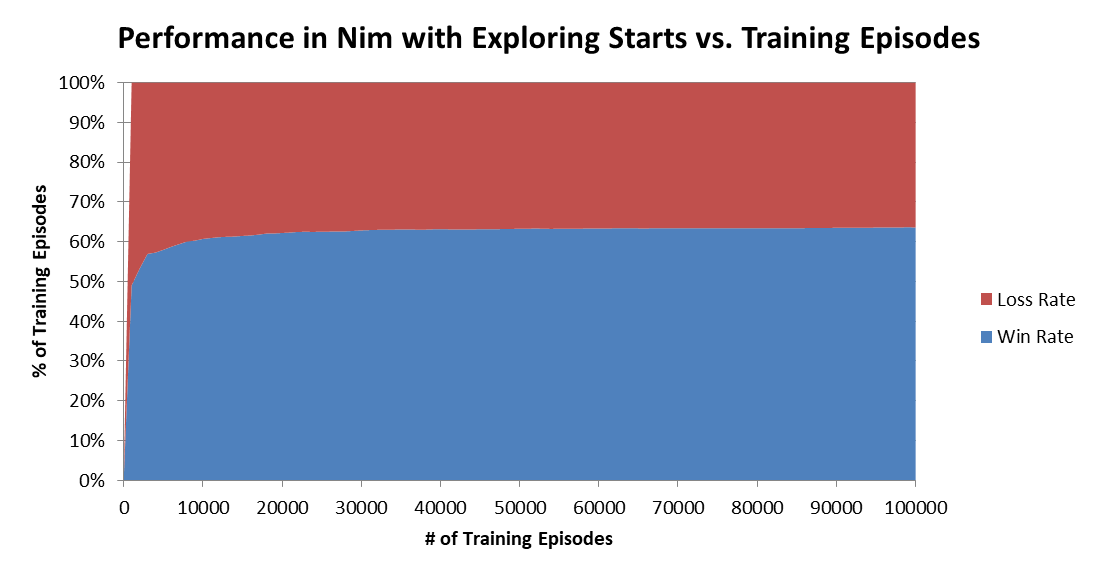
\includegraphics[width=125mm]{NimExploringStarts_Convergence.png}
		\caption{Changes in agent's performance in Nim with exploring starts}
		\label{nim-exploring-starts-convergence}
	\end{center}
\end{figure}

The policy converges after around 14,000 training episodes and at that point the winning rate is 61.3\% and the number of states encountered is 511 (i.e. all states). This is very interesting because in the convergence experiment with the on-policy $\varepsilon$-soft MC agent, the largest winning rate \emph{at the point when the agent's policy converges} of any value of $\varepsilon$ (among the values in Table \ref{table:nim_convergence_table}) was around 76.5\%, meaning it won 15\% more training episodes than the exploring starts agent.

[\emph{I will add more discussion here. I could also make the two agents *after all the training* play another 100,000 games and see who wins more.}]


%-----------------------
\chapter{Discussion}

\section{Learning Optimal Epsilon}

[\emph{Discussion of how I tried this but it didn't really work conceptually.}]

\section{Alternative Implementations of Symmetry-Breaking}

Another way of eliminating symmetry in Tic-Tac-Toe was also considered: limiting the actions available from each state such that no two actions result in symmetrical states. An interesting result of this idea is that it would slightly alter the way the game is played. Suppose a random agent is asked to select a move from the game's initial state (i.e. empty grid). In the Normal implementation, there are nine possible actions: putting an \textbf{X} token in one of the nine grid cells. In this ``Limited Actions'' version, there are only three possible actions: putting an \textbf{X} token in a corner, in the middle of the grid, and in the middle of one of the sides. To give a specific example of how this would change the game, notice that the probability of the agent choosing the action that involves placing their token in the middle of the grid is $\frac{1}{9}$ in the Normal implementation and $\frac{1}{3}$ in the Limited Actions version. Thus, the agent will end up choosing this action three times as frequently in the latter version.

In the limit of infinitely many games, however, the MC agent would encounter all states and choose all possible moves an equal number of times, thus computing an accurate expected return for each action. It would be interesting to compare the performance of such a Limited Actions implementation with the Symmetric Equality implementation. Both should perform equally well on any game given enough training, but it is possible that they might improve at different rates.


\section{More... to be discussed}


%-----------------------
\chapter{Conclusion}


\section{Future Work}


\section{Personal Reflections}

This has been a really great learning experience, not only in terms of discovering the field of reinforcement learning and its applications, but also in terms of gaining experience with building up a large, complex programming project from scratch using a variety of technical tools.

When I was in high school, I designed and implemented the classic board game Nine Men’s Morris where a user plays against an algorithm I wrote. My plan for the project was to ask my friends and family to play my game and to store the moves made in each game so that I could build up a database of sequences of moves and outcomes of the game. I hoped to somehow compute which moves were the best and get my algorithm to learn which moves made winning the most likely. Little did I know, I wanted to invent RL from scratch – unaware of its existence or of the amount of research in the field. Several years later, I am delighted to have had the chance to work on a similar project, but this time on a deeper level using well-known computational algorithms. [\emph{I don't know if this paragraph should stay in my final version...}]

When I started working on this project, I decided to treat it as an opportunity to develop many skills that are critical for a career in software engineering:

\begin{itemize}
	\item Writing clean, maintainable, well-documented code
	\item Designing and implementing tests for my code
	\item Using a build tool to manage dependencies between packages in my project as well as with external libraries
	\item Using version control effectively
\end{itemize}

I tested the methods in my API using a unit-testing framework for Java called JUnit. I also used a testing framework for Java called Mockito – this allowed me to verify the behaviour of objects with external dependencies by creating “mock objects” for theses dependencies, which mimic real objects but do so in a particular way that I can specify.

In order to save my experiment results in a format that would facilitate the creation of graphs, I used opencsv, a CSV parser library for Java.

To manage my project’s dependencies, I used a build tool developed by Google called Bazel and I used Git for version control.

Overall, I really enjoyed learning about RL algorithms and exploring their applications and success rates, all while developing strong programming skills that will help me throughout my career.


%--------------------------------
\chapter{Acknowledgements}



%--------------------------------
\bibliography{mybib}{}
\bibliographystyle{plain}

\end{document}
